\documentclass[10pt,conference,compsocconf]{IEEEtran}

\usepackage{hyperref}
\usepackage{graphicx}	% For figure environment
\usepackage{amsmath}


\begin{document}
\title{Machine Learning project : Higgs Challenge}

\author{
  Antonio Morais, Cedric Maire and Benjamin D\'el\`eze \\
  \textit{Master in computer and communication sciences, EPF Lausanne, Switzerland}
}

\maketitle

\begin{abstract}
  Named after physicist Peter Higgs the Higgs boson is an elementary particle produced by the quantum excitation of the Higgs field. Its existence was first suggested in 1964 and confirmed at CERN in 2012. The tackled challenge was to predict if an event is in fact a Higgs boson or background noise. Generated data sets in experiments are often highly dimensional, complex and hard to analyse or interpret. Machine learning techniques are often used to undergo this complexity and try to classify data using different techniques. Using different algorithm and data processing we managed to achieve more than 80\% of correctness on a given test data set.
\end{abstract}

\section{Introduction}

The aim of this project is to do the Higgs Boson challenge which is a challenge organized by the ATLAS physicists and data scientists from the CERN \cite{higgsChallenge14}. In this challenge, the goal was the improvement of the course of actions that is producing the selection region. To do so, a data set was given with information about different parameters which could induce the presence or not of a the boson of Higgs. The objective of this project was then to determine, depending on different data that was retrieved, if there is possibly a boson of Higgs.

In order to determine whether there is a boson of Higgs or not we had to implement different methods used in machine learning that we got to learn in the CS-433 Machine Learning course given at EPFL \cite{MLcourse18}. All of these methods could solve in part this problem but the real objective was to improve the result given by these different methods. To do so there was a few different ways, for example we could use cross-validation to be able to test different stuff and if it was improving the algorithm or we could also do some data-cleaning to reduce the different outliers and use them to our advantage.

\section{Models and Methods}

There was different methods that we had to implement to be able to improve the methods that were solving the problem given by the Higgs challenge \cite{higgsChallenge14}. These different methods are

\begin{description}
\item[Build polynomials] \ \\
As we have seen in the course one of the basic improvement methods for machine learning is the build polynomial method \cite{MLcourse18}. In this method, we take each column of the data set and we extend it with n different columns (where n is the degree to which we want to elevate the column) and the n different columns are the column of the data set elevated to different degrees from 0 to n. Here's an example of what this method should return for a degree 3 : 

\begin{center}
$Entry : 
\begin{pmatrix}
 1 \\
 2 \\
 3 
\end{pmatrix}
$
$Return : 
\begin{pmatrix}
 1&1&1&1 \\
 1&2&4&8 \\
 1&3&9&27 
\end{pmatrix}
$
\end{center}
 
 The improvement done when using this method was really impressive, it was an improvement of around 3\%

\item[Cross validation] \ \\
We also saw in class that a good way to be able to improve our percentage was to do cross validation to see if a certain method was improving or not the correctness of our methods \cite{MLcourse18}. Cross validation is a method that divides the train set in n different sets and will train with n-1 sets and test with the remaining set and it will do this for all the different sets. Doing so we can observe the percentage of correctness of our method and be sure that we are not regressing.

\item[Correlated features] \ \\
One of the ideas that we had in order to improve our method was to find the correlation that there was between the different features and the label \cite{brown14}. Doing so we could remove the ones that were the less correlated, even if it was not causality it could improve the result. The different correlation that we found can be found in Figure~\ref{fig:corr-coefs}. Sadly when removing the different columns that were almost not correlated, the result didn't improve at all, it even lowered sometimes.

\begin{figure}[hbtp]
  \centering
  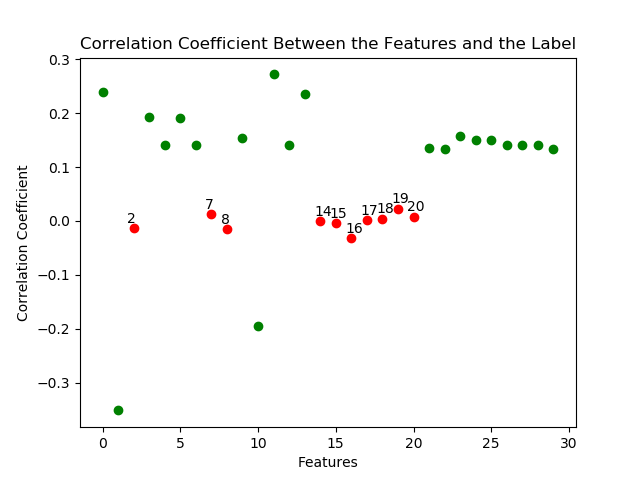
\includegraphics[width=\columnwidth]{images/corrcoefs.png}
  \caption{Correlation between the features and the label.}
  \vspace{-3mm}
  \label{fig:corr-coefs}
\end{figure}

\item[Setting the -999 to another value] \ \\
Another idea that we got was to replace the undefined values by some other values of our choice to simulate as if it was "normal" values. We tested different values : 0, the mean of the defined values and the median of the defined values. All of them improved our method of around 0.5 to 1\%. But finally, we decided to do something else with the undefined values as it will be explained in the next point.

\item[Different sets] \ \\
While reading the information that was given about the data set  \cite{higgschallenge14}, we noticed that a lot of features were actually depending on the PRI\_jet\_num feature. For example, all but one features that could be undefined were directly depending on the value of PRI\_jet\_num. So we decided to separate the data set in several smaller sets to have better weights for these specific sets \cite{brown14}. The PRI\_jet\_num feature can have 4 different values (0, 1, 2 and 3) and the only feature that could be undefined without depending on the PRI\_jet\_num feature is the DER\_mass\_MMC feature. So we decided to do 8 sets as shown in the tree in Figure~\ref{fig:tree-sets}. 

\begin{figure}[hbtp]
  \centering
  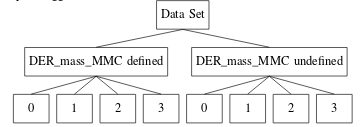
\includegraphics[width=\columnwidth]{images/treeSets.png}
  \caption{All the different sets we did, the numbers are the values of the PRI\_jet\_num feature}
  \vspace{-3mm}
  \label{fig:tree-sets}
\end{figure}

This way of separating the data in different sets improved the result of approximately 3\%

\end{description}

\section{Results and discussion}

So the two methods that really improved our percentage of correctness are the separation of the data into different sets and the build polynomials method. What we did to see the correctness in the following results is that we trained with the training set and then we predicted the y for the same training data set and computed the correctness by comparing them to the real y. 

\begin{table}[h]
\centering
  \begin{tabular}[c]{|l||c|c|c||c|}
    \hline
    Method&$\lambda$&$\gamma$&max iterations&percentage\\
    \hline
    least\_squares\_GD&-&0.2&1000&76.49\%\\
    \hline
    least\_squares\_SGD&-&0.005&1000&74.79\%\\
    \hline
    least\_squares&-&-&-&76.49\%\\
    \hline
    ridge\_regression&0.1&-&-&76.02\%\\
    \hline
    logistic\_regression&-&0.001&1000&74.80\%\\
    \hline
    reg\_logistic\_regression&0.001&0.001&1000&74.80\%\\
    \hline
  \end{tabular}
  \caption{Percentage of correctness for the implemented methods with the separation in different sets.}
  \label{tab:per-sets}
\end{table}

As we can see in Table~\ref{tab:per-sets} using the different sets improved almost all methods of around 3\% as before the correctness was around 73\%. We will now use also the build polynomials method with a degree of 3 to show a beginning of improvement, of course, afterwards, we did different tests to find the best combination of parameters of the best method and degree of the build polynomial method.

\begin{table}[h]
\centering
  \begin{tabular}[c]{|l||c|c|c||c|}
    \hline
    Method&$\lambda$&$\gamma$&max iterations&percentage\\
    \hline
    ridge\_regression&0.1&-&-&79.57\%\\
    \hline
    logistic\_regression&-&0.001&1000&77.88\%\\
    \hline
    reg\_logistic\_regression&0.001&0.001&1000&77.88\%\\
    \hline
  \end{tabular}
  \caption{Percentage of correctness for the implemented methods with the separation in different sets and a degree of 3 for the build polynomials method.}
  \label{tab:per-sets-poly}
\end{table}

Due to our implementations, the different least\_squares methods weren't working when using build polynomials but as the ridge\_regression was already pretty good, we assumed that we could concentrate our work on this function. And as we can see in Table~\ref{tab:per-sets-poly}, there was also a pretty good improvement of around 3\%.

In order to find the best parameters, we ran an algorithm that tested the ridge\_regression algorithm with different lambdas and different degrees to deduce what was the best combination for each different set. Doing so, we managed to have 81.95\% of correctness when doing cross validation.

\section{Summary}

In this project, we managed to implement different methods that could solve this machine learning problem. Doing so, we figured out that one important aspect of machine learning is preprocessing the data and when doing so we could really improve the results given by the first implementations. we also saw that for this type of data the ridge\_regression was the best algorithm and reg\_logistic\_regression was also pretty good but slower to compute so that's why we preferred the ridge\_regression one.

\bibliographystyle{IEEEtran}
\bibliography{ML2LaMort-literature}

\end{document}
